% =============================================================================
% APPENDIX B: COMPLETE ClimVaR METHODOLOGY
% Based on Epelbaum (2025). Trimmed for whitepaper: full derivations
% deferred to the original reference.
% =============================================================================
\newpage
\section{ClimVaR Methodology} \label{sec:climvar-full}

% Color definitions needed for figures in this appendix
\definecolor{BLUE_MAIN}{RGB}{0, 102, 161}
\definecolor{BLUE_PASTEL}{RGB}{55,127,171}
\definecolor{RED_MAIN}{RGB}{227, 114, 88}
\definecolor{RED_PASTEL}{RGB}{164,98,76}
\definecolor{RED_PASTEL_2}{RGB}{231, 143, 115}
\definecolor{RED_DARK}{RGB}{196,172,107}
\definecolor{GREEN_MAIN}{RGB}{146, 178, 119}
\definecolor{GREEN_DARK}{RGB}{109, 142, 81}
\definecolor{GREEN_DARKER}{RGB}{73, 95, 54}
\definecolor{GREEN_REL}{RGB}{64, 130, 109}
\definecolor{BROWN_MAIN}{RGB}{194, 144, 124}
\definecolor{BROWN_DARK}{RGB}{163, 98, 84}
\definecolor{GOLD_MAIN}{RGB}{238, 232, 170}
\definecolor{GOLD_DARK}{RGB}{255, 219, 88}

% Macro definitions for Expected Shortfall plots
% fillbetween library loaded in preamble
\def\oe9{1e9}
\def\sig1{sqrt(0.2)*\oe9}
\def\sig2{sqrt(0.1)*\oe9}
\def\sig3{sqrt(0.3)*\oe9}
\def\muC{2}
\def\sigC{sqrt(0.5)*\muC}
\def\sigLsq{ (\sigC/\muC)^2 + ((\sig1+\sig2+\sig3)/\oe9)^2 + (\sigC/\muC)^2*((\sig1+\sig2+\sig3)/\oe9)^2 }
\def\muL{\muC*\oe9}
\def\muLlog{ln(\muL/sqrt(1+\sigLsq))}
\def\sigL{sqrt(ln(1+\sigLsq))}
\def\sigD{sqrt( (\sig1+\sig2+\sig3)^2 )}
\def\sigDcv{ \sigD/\oe9 }
\def\muDlog{ln(\oe9/sqrt(1+\sigDcv^2))}
\def\sigS3sq{ (\sigC/\muC)^2 + ((\sig1+\sig2)/\oe9)^2 + (\sigC/\muC)^2*((\sig1+\sig2)/\oe9)^2 }
\def\muS3log{ln(\muL/sqrt(1+\sigS3sq))}
\def\sigS3{sqrt(ln(1+\sigS3sq))}
\def\sigBothsq{ ((\sig1+\sig2)/\oe9)^2 }
\def\muBothlog{ln(\oe9/sqrt(1+\sigBothsq))}
\def\sigBoth{sqrt(ln(1+\sigBothsq))}

\tikzset{
    declare function={
        norminv(\p)=sqrt(-2*ln(1-\p))-(2.515517+0.802853*sqrt(-2*ln(1-\p))+0.010328*(-2*ln(1-\p)))/(1+1.432788*sqrt(-2*ln(1-\p))+(0.189269+0.001308*sqrt(-2*ln(1-\p)))*sqrt(-2*ln(1-\p)))*sqrt(-2*ln(1-\p));
        normcdf(\x)=1/(1+exp(-1.6545*\x*(1+0.25*\x)));
    }
}
% \CDF operator not needed — "CDF" used as plain text

\subsection{Introduction} \label{sec:intro}

Climate change is one of the central problem humanity has to tackle in the 21st century. The frequency of extreme climate events is already increasing, and this tendency can only worsen if no action is taken to limit anthropic carbon emissions. In recent years, several climate/financial regulation frameworks \cite{EUC}-\cite{Deloitte} were developed, aiming at collecting climate related data and be somewhat prescriptive \cite{EuropeanClimateLaw} on how to decarbonate. Nevertheless, the current accounting norms (GAAP, IFRS...) do not even fully capture simple materiality aspects, making relevant financial decisions at public and private level difficult.

\vspace{0.2cm}

As we will see in section \ref{sec:related}, several studies have been done in the past years on the financial impact  caused by some climate risks. But most of these studies focus on one aspect of the problem: a specific transition risk \cite{Transition1} like carbon cost \cite{Adenot}\cite{RoncalliCC} or litigation \cite{Litigation1}\cite{Litigation2}, nature risk \cite{NatureF1}\cite{NatureF2}\cite{NatureF3}\cite{RoncallliBiodivBook}\cite{RoncalliNatureCap}, or physical climate risk \cite{LeGuenedal}. 


\vspace{0.2cm}

A unifying approach is therefore somewhat lacking, though most of the tools needed to get there have already been developed. 

\vspace{0.2cm}

In this paper we will use a standard Discounted Cash Flow (DCF) approach to cover all the major climate risks to be faced in the years/decades to come.

\vspace{0.2cm}

Our aim is to help public and private organisms measure the economic viability of systems. Five types of systems will be studied: 
\begin{itemize}
\item[•] A portfolio of financial products.
\item[•] A company.
\item[•] An entity within a company.
\item[•] A site of an entity\footnote{We consider in all the following an entity to be a company part belonging to a specific country and operating within a specific sector of activity.}.
\item[•] A company product (depending on several sites). A product is produced on several sites, and one site can produce several products.
\end{itemize}

\vspace{0.2cm}

Having access to better financial assessments of systems should allow for a better resilience of the economic actors with respect to climate change, and should ease the transformations needed to fight it: decarbonate the supply chain, build floodgates, avoid brown sectors when it makes sense...

\vspace{0.2cm}

Our objective will be reached if regulators, auditors, public and private actors can start using the white box formalism that we (though obviously building a lot on existing works) develop in the next sections. This should help them really assess the economic profitability of the projects/systems they supervize by duly accounting for climate change.

\vspace{0.2cm}

As already stated, we will adapt a standard DCF approach to estimate the future valuation $V$ of a system. In all the following, the system can be one of the fives already stated. We will augment the traditional DCF approach by considering variations related to climate. These variations can be related to 
\begin{itemize}
\item[$\bullet$] physical risk: flood, drought, wildfire \cite{IPPC1}\cite{IPPC2}...
\item[$\bullet$] transition risk: carbon tax, customer shift  \cite{Adenot}\cite{RoncalliCC}\cite{Bouchet}\cite{NGFS1}..
\item[$\bullet$] nature risk: loss of nature capital \cite{RoncalliNatureCap}
\end{itemize}

We call our central DCF formula embedding climate risks ClimVaR (for Climate Value at Risk)

\vspace{0.2cm}

The rest of this note is devoted to deriving ClimVaR for the five systems already mentioned.  It is organized as follows. Section~\ref{sec:related} discusses related work, insisting on the fact that the current paper builds on existing (but siloed) studies. Section~\ref{sec:notation} regroups all notations. The tools developed in this paper are not advanced, but put together they cover a large range of concepts. The reader should therefore refer to this section to understand the approach and all symbols. Section~\ref{sec:climvar} presents the central result of this work: a valuation formula encompassing physical and transition climate-related effects. Section~\ref{sec:climvar-terms} summarizes the derivation of individual loss terms, referring the reader to \citet{epelbaum2025} for the complete mathematical treatment. Section~\ref{sec:scenario} elaborates on the scenario and uncertainty topic. The link with the usual Value At Risk (VaR) is also made. The financially knowledgeable reader pondering on the use of the ClimVaR term will benefit from \ref{sec:shortfall}. Adaptation strategies and their economic merit are discussed in the main text (Chapter~III, Finding~4). Extensions to additional transition risks (reputation, litigation, technology, investor sentiment) are deferred to subsequent work.


\subsection{Related work} \label{sec:related}

Relating climate risks to financial impacts is not a new topic, but it has seen a rise of interest in recent years.

\vspace{0.2cm}

The climate/economy relationship could be traced back to the Meadows Report \cite{Meadows1972}, which initiated the works on Integrated assessment Models (IAMs), coupling classical macro-economic equations with exogenous (climate, but not only) economic data. Following its steps, numerous IAMs \cite{DICE}\cite{GLOBIOM}\cite{Remind}\cite{MESSAGE} were developed in the past 50 years, adding among other things local (by opposition to world or large regions) and sectoral modelling.

\vspace{0.2cm}

Climate risks could loosely be divided into 3 different categories:
\begin{itemize}
\item[•] Physical risk \cite{IPCCRisk} correspond to the impact of climate events on human activity: a strong wind damaging a building, a flood interrupting business activities...  Several papers \cite{LeGuenedal}\cite{BID}\cite{Bernhofen}\cite{Azzone} have investigated the impact of these physical events onto financial activities.
\item[•] Nature (biodiversity) risk is a more recent center of interest. It analyzes the effect of nature/ecosystem/biosphere degradation onto economic activities \cite{RoncalliNatureCap}\cite{SPGNatureBio}\cite{NatureF4}. As we are approaching several planetary limits \cite{PlanetaryBoundaries}\cite{PlanetaryBoundariesUpdate}, this topic should see intense activities in the years to come.
\item[•] Transition risk represents the human adaptation to climate change, in the forms of laws, norms, bans, taxes, individual consumer behaviours... It may be the topic that have been the focus of the most attention in the past decade \cite{RoncalliCC}\cite{TransitionRiskCaldecott}\cite{FDIC}\cite{TCFD}, but recent changes in international geopolitics \cite{OmnibusRollback} could make this risk less pregnant than the physical one in the years to come.
\end{itemize}

Some paper on Climate Value At Risk \cite{RoncalliVaR}\cite{MSCIClimateVaR} already exist, but they do not yet offer a unifying, quantitative, white box analysis encompassing all the risks previously mentionned. The present work aims to do just so.

\subsection{Notation} \label{sec:notation}

\subsubsection{Generic concepts}

\begin{itemize}
\item[•] $t$: times. In the present paper year is the time unit, unless specified otherwise.
\item[•] $\nu$: Scenario (more on scenarios in section \ref{sec:scenario-inter})
\item[•] $\lambda$: Intra scenario uncertainty (more on it and link with VaR in section \ref{sec:scenario-intra}).
\item[•] $r$: Supply chain rank. $0$ means direct operation (i.e. a system direcly operated by the project leader). $1$ means direct supplier (meaning supplier to which the project leader directly buys). $1+$ means all suppliers (direct and indirect. Indirect suppliers are suppliers of suppliers, suppliers of suppliers of suppliers... And so on). $0+$ means all contributions, direct and suppliers.
\end{itemize}

\subsubsection{Company related concepts}

We will denote
\begin{itemize}
\item[•] $FP$: Financial Portfolio.
\item[•] $C$: Company (possibly part of for a financial portfolio).
\item[•] $E$: Entity of a company.
\item[•] $S$: Site of an entity. We will interchangeably use assets $a$.
\item[•] $P$: Product.
\item[•] $c$: World countries.
\item[•] $s$: Activity sectors. we take the ISIC standard \cite{ISIC} for encoding the activity sectors, and consider the 45 ISIC sectors used in the 2023 OECD work \cite{OECD1}\cite{OECD2} unless stated otherwise.
\item[•] $S^{(1)}$: Carbon equivalent emissions  within a year corresponding to direct system actitivities, called Scope 1 \cite{S1} in the litterature.
\item[•] $S^{(2)}$: Carbon equivalent emissions within a year corresponding to system electricity consumptions, called Scope 2 \cite{S2} in the litterature.
\end{itemize}


\subsubsection{Financial concepts}

We will note

\begin{itemize}
\item[•] $V$: Valuation.  
\item[•] $\text{VaR}$: Valuation At Risk.
\item[•] $FCF$: Future Cash Flow. .
\item[•] $T$: Terminal time value.
\item[•] $g$: Perpetual growth rate.
\item[•] $g^{(t)}$: Yearly growth rate.
\item[•] $Y$: System gross revenues. 
\item[•] $\omega$ (or $W\!ACC$): Weighted Average Cost of Capital. $\omega$ will be preferred in equations. $W\!ACC$ variation is deferred to future work.
\item[•] $DCF$: Discounted Cash Flow. $DCF^{(t)}=FCF^{(t)}/\left(1+\omega\right)^t$. 
\item[•] $COGS$: Cost Of Goods Sold.
\item[•] $c$: $COGS$ to Revenue ratio.
\item[•] $OPEX$: Operating Expenses.
\item[•] $o$: $OPEX$ to Revenue ratio.
\item[•] $s$: Salary to Revenue ratio. 
\item[•] $P$: Absolute (monetary) system purchases will be noted as $P$.
\item[•] $p$: system purchases ratio will be noted as $p$, and we consider $p=c-s$. 
\item[•] $so$: Outdoor salary mass to Revenue ratio.
\item[•] $si$: Indoor salary mass is not used in the present analysis. Obviously $s=si+so$.
\item[•] $e$: Electricity expenses to Revenue ratio.
\item[•] $ec$: Electricity cooling expenses to Revenue ratio.
\item[•] $\tau$: system (federal) tax rate.
\item[•] $CFO$: Cash Flow from Operation.
\item[•] $CAPEX$: CAPital EXpenditures.
\item[•] $NWC$: for Net Working of Capital. 
\item[•] $DA$: for Depreciation (and Amortization)\footnote{In our approach we follow the Generally Accepted Accounting Principles (GAAP)\cite{KPMG}, which are for instance somewhat different from the French accounting formalism.}. 
\item[•] $k$: for $CAPEX$ over Revenue ratio. 
\item[•] $n$: for $NWC$ over Revenue ratio. 
\item[•] $d$: for $DA$ over Revenue ratio. 
\item[•] $op$: Operating Profit over Revenue Ratio. $op=1-c-o$.
\item[•] $i$: Insurance premium.
\item[•] $AV$: Asset Value (in the sense of hard assets: buildings...).
\end{itemize}

\subsubsection{Climate risk related concepts}

\begin{itemize}
\item[•] $cc$: Climate change (by contrast with quantities computed without considering it).
\item[•] $h$: Climate hazard (drought, flood, wild fire...).
\item[•] $\sigma$: Customer shift.
\item[•] $\beta$:  Business Interruption Days (BID) (as a fraction of year) at country sector level.
\item[•] $\chi$:  Business Interruption Days (BID) at asset site level.
\item[•] $\rho$: Degradation of renewable nature capital (as a \% of revenue).
\item[•] $\delta$: Damages on assets (as a \% of asset value).
\item[•] $CC^{(i)}$: Carbon costs related to scope $i$.
\item[•] $\xi$: Heat Productivity Loss \cite{HI1}\cite{HI2}\cite{HPL1}\cite{HPL2}\cite{HPL3}.
\item[•] $\gamma$: Cooling cost increase \cite{CDD} (from a reference to a future time period).
\end{itemize}

\subsubsection{Multi Regional Input Output table (MRIOT) related concepts}

MRIOT is a rich topic on its own, that we only minimally cover in this paper to the extent of our need.

\begin{itemize}
\item[•] $Z_{_{cs,c's'}}$: Multi Regional Input Ouput Table (MRIOT). Following \cite{MillerMRIOT}, we adopt the convention where rows of $Z$ correspond to suppliers and columns to clients. $Z_{_{cs,c's'}}$ is therefore a financial flux within a year\footnote{Usually in USD or M~USD.} between sector $s'$ of country $c'$, buying goods from  sector $s$ of country $c$.
\item[•] $X_{_{cs}}$: Total financial output of sector $s$ of country $c$. 
\item[•] $A_{_{cs,c's'}}$:  $A$ Technical coefficient matrix. Coefficients as $A_{_{cs,c's'}}=Z_{_{cs,c's'}}/X_{_{c's'}}$.

\item[•] $L_{_{cs,c's'}}$:  Leontief matrix. $L=\mathbb{I}+ A^T+\left(A^T\right)^2+\cdots= \left(\mathbb{I}-A^T\right)^{-1}$.
\end{itemize}

\subsubsection{Carbon cost related concepts}

We will use the following notations

\begin{itemize}
\item[$\bullet$] $C^{(t)}_{_c}$: "Raw" carbon price (as USD per tons of CO2 equivalent emissions, or TCO2e). Carbon prices \cite{WorldBankCC} are given at country level and are considered time dependent.
\item[$\bullet$] $F^{(t)}_{_s}$: Free allocation rates. These are sectoral allocations that allow sectors to discount part of their carbon costs. In our approach, Free allocations are always present in Business as Usual scenarios and removed after 2030 for other ones. More on scenarios in section \ref{sec:scenario}.
\item[$\bullet$] Passthrough $P_{_s}$ at sector level. Considered to be $1$ for the remaining of this paper. This is a strong assumption that we will relax in future studies.
\item[$\bullet$] $\mathcal{C}^{(t)}_{_{cs}}$: Combined "Raw" carbon price. $\mathcal{C}^{(t)}_{_{cs}}=F^{(t)}_{_s}C^{(t)}_{_c}P_{_s}=F^{(t)}_{_s}C^{(t)}_{_c}$.
\item[$\bullet$] $I^{(i)}_{_{cs}}$: Carbon intensities (TCO2e per revenue (USD)) for scope $i$. When $i$ is unspecified, it is for scope 1. These country sector intensities can be evaluated in several manners: having access to database of company emissions + financial data \cite{CDP}, or a MRIOT approach (like the one performed by Exiobase \cite{Exiobase})...
\end{itemize}

\subsection{ClimVaR model} \label{sec:climvar}

We leave aside the notion of scenario and uncertainty for the time being. We will come back on these important topics in section \ref{sec:scenario}. As is standard in valuation approaches, ClimVaR will take major financial information from income statements, balance sheets and cash flows to form the Discounted Cash Flow. ClimVaR novelty resides in how it computes and aggregates climate risk effects on different parts of the Discounted Cash Flow. As stated in section \ref{sec:intro}, we want to derive these effects for five systems (from the finer to the coarser level): products, sites, entities, companies, financial portfolios. As we will see in the following, financial portfolios can be seen as the aggregation of company valuation computations, and the same goes for entities with respect to companies and sites with respect to entities. The relation is not one to many but many to many for products to sites valuation: a product is generally produced by several sites, but sites usually also produce parts of several products at once.

\vspace{0.2cm}

We will start with the entity computation, that is the simpler to explain on its own. From it we will trivially derive ClimVaR formulas for companies and financial portfolios. We will then explain the adaptations needed on the entity formula to get the sites and finally the product ones.

\subsubsection{Entity ClimVaR} \label{sec:climvar-entity}

\vspace{0.2cm}

A DCF model \cite{Kruschwitz}\cite{Valuation} estimates the current value (at current time $0$) of a system as the sum of it's future Discounted Cash Flows. We first focus our attention on an entity, belonging to a sector $s$ of a country $c$. Valuation reads there

\begin{align}
V^{(E)}_{_{cs}}&=\sum_{t=1}^{+\infty}\frac{FCF^{(t)}_{_{cs}}}{(1+WACC_{_{cs}})^t}\;,\label{eq:base-val}
\end{align}

where $W\!ACC$ is assumed to be time/climate independant and equal to $\omega_{_{cs}}$. 

\vspace{0.2cm}

It is good practice to take a terminal value year $T$ (which we consider constant at company level), after which the system is experiencing fixed perpetual growth (Gordon Growth Model) $g_{_{cs}}$. 

\begin{align}
V^{(E)}_{_{cs}}&=\sum_{t=1}^{T}\frac{FCF^{(t)}_{_{cs}}}{\left(1+\omega_{_{cs}}\right)^t}
%
+\frac{FCF^{(T)}_{_{cs}}}{\left(1+\omega_{_{cs}}\right)^t}\frac{1+g}{\omega_{_{cs}}-g_{_{cs}}}\;.
\end{align}
To simplify the notation, we will take 
\begin{align}
FCF^{(T+1)}_{_{cs}}&=FCF^{(T)}_{_{cs}}\frac{(1+g_{_{cs}})(1+\omega_{_{cs}})}{(\omega_{_{cs}}-g_{_{cs}})}\;,\label{eq:perpetfcf}
\end{align}
so that
\begin{align}
V^{(E)}_{_{cs}}&=\sum_{t=1}^{T+1}\frac{FCF^{(t)}_{_{cs}}}{\left(1+\omega_{_{cs}}\right)^t}\;.
\end{align}

\vspace{0.2cm}

In our model, we will be interested by the Climate Value at Risk (ClimVaR) \cite{Kruschwitz}\cite{Valuation}\cite{Damodaran1}: namely the difference between a valuation without and with climate change. This is the central quantity that we want to estimate

\begin{align}
\text{VaR}^{(E)}_{_{cs}}&=\Delta V^{(E)}_{_{cs}}=V^{(E)}_{_{cs}}-V^{(E,cc)}_{_{cs}}
%
=\sum_{t=1}^{T+1}\frac{FCF^{(t)}_{_{cs}}-FCF^{(t,cc)}_{_{cs}}}{\left(1+\omega_{_{cs}}\right)^t}\;.\label{eq:var}
\end{align}

To be noted, we will also be interested by a $\delta$VAR, namely

\begin{align}
\delta \text{VaR}^{(E)}_{_{cs}}&=\frac{\Delta V^{(E)}_{_{cs}}}{V^{(E)}_{_{cs}}}\;,\label{eq:delta-var}
\end{align}

that estimates the share of the total value at risk\footnote{Keep in mind that the climate can generate value, in the case of customer shift for instance.}.

\vspace{0.2cm}

The FCF at time $t$ reads \cite{Damodaran1}

\begin{align}
FCF^{(t)}_{_{cs}}&=CFO^{(t)}_{_{cs}}- CAPEX^{(t)}_{_{cs}} - \delta NWC^{(t)}_{_{cs}}\;,
\end{align}


In a first approach, we will assume that both $NWC$ (corresponding to short term assets and liabilities cash fluxes) and $CAPEX$ do not depend on climate change (as we will see, we will consider fixed assets accelerated degradation because of climate change via the OPEX term in CFO. To be noted $CAPEX$ will play a role when taking into account climate actions), and that they represent a constant fraction of revenues $Y$:

\begin{align}
\delta NWC^{(t)}_{_{cs}}&=
%
NWC^{(t)}_{_{cs}}- NWC^{(t-1)}_{_{cs}}\approx
%
 n_{_{cs}}\left(Y^{(t)}_{_{cs}} - Y^{(t-1)}_{_{cs}}\right)\;,\notag\\
%
CAPEX^{(t)}_{_{cs}} & \approx k_{_{cs}}Y_{_t}\;.
\end{align}

In that case

\begin{align}
\text{VaR}^{(E)}_{_{cs}}&=\sum_{t=t_0+1}^{T+1}\frac{CFO^{(t)}_{_{cs}}-CFO^{(t,cc)}_{_{cs}}}{(1+w)^t}\;.
\end{align}

$CFO$ reads

\begin{align}
CFO^{(t)}_{_{cs}}&=NOPAT^{(t)}_{_{cs}}+DA^{(t)}_{_{cs}}\notag\\
%
&=\left[Y^{(t)}_{_{cs}}-COGS^{(t)}_{_{cs}}-OPEX^{(t)}_{_{cs}}-DA^{(t)}_{_{cs}}\right]
%
\left[1-Tax^{(t)}_{_{cs}}\right]+DA^{(t)}_{_{cs}}\;,
\end{align}

In our model, we assume that taxes are not affected by climate change\footnote{We will see later that Carbon Taxes are taken into account via the Revenue and the OPEX channel} and are constant ($\tau_{_{cs}}$) through time. In addition, we also assume that $DA$ is not affected by climate change (again, additional costs incured to repair buildings will be considered as OPEX) and is a constant share of the total revenue
\begin{align}
DA^{(t)}_{_{cs}}&\approx d_{_{cs}} Y^{(t)}_{_{cs}}\;.
\end{align}

We therefore focus our attention on the Operating profit

\begin{align}
OP^{(t)}_{_{cs}}&=Y^{(t)}_{_{cs}}-COGS^{(t)}_{_{cs}}-OPEX^{(t)}_{_{cs}}\;.\label{eq:profit}
\end{align}

And our central climate VAR (\ref{eq:var}) becomes
\begin{align}
\text{VaR}^{(E)}_{_{cs}}&=
%
\sum_{t=1}^{T+1}\frac{1-\tau_{_{cs}}}{\left(1+\omega_{_{cs}}\right)^t}\left[OP^{(t)}_{_{cs}}-OP^{(t,cc)}_{_{cs}}\right]\notag\\
%
&=\sum_{t=1}^{T+1}\frac{1-\tau_{_{cs}}}{\left(1+\omega_{_{cs}}\right)^t}\left[
%
Y^{(t)}_{_{cs}}-Y^{(t,cc)}_{_{cs}}-\left(COGS^{(t)}_{_{cs}}-COGS^{(t,cc)}_{_{cs}}\right)
%
\right.\notag\\
%
&\left.  -\left(OPEX^{(t)}_{_{cs}}-OPEX^{(t,cc)}_{_{cs}}\right)\right]\;.
\end{align}

We continue our modelling by assuming that $COGS$ and $OPEX$ are proportional to revenues \cite{Damodaran3}
\begin{align}
COGS^{(t)}_{_{cs}}&\approx c_{_{cs}} Y^{(t)}_{_{cs}}\;,&
%
OPEX^{(t)}_{_{cs}}&\approx o_{_{cs}} Y^{(t)}_{_{cs}}\notag\\
%
COGS^{(t,cc)}_{_{cs}}&\approx c^{(t,cc)}_{_{cs}} Y^{(t,cc)}_{_{cs}}\;,&
%
OPEX^{(t,cc)}_{_{cs}}&\approx o^{(t,cc)}_{_{cs}} Y^{(t,cc)}_{_{cs}}\;,
\end{align}
so that, recalling that
\begin{align}
op_{_{cs}}&=1- c_{_{cs}}-o_{_{cs}}\;,
\end{align}
we get
\begin{align}
\text{VaR}^{(E)}_{_{cs}}=\sum_{t=1}^{T+1}\frac{1-\tau_{_{cs}}}{\left(1+\omega_{_{cs}}\right)^t}&\left[
%
op_{_{cs}}\left(Y^{(t)}_{_{cs}}-Y^{(t,cc)}_{_{cs}}\right)\right.\notag\\
%
&\left. +\left(c^{(t,cc)}_{_{cs}}- c_{_{cs}}\right)Y^{(t,cc)}_{_{cs}}
%
+\left(o^{(t,cc)}_{_{cs}}- o_{_{cs}}\right)Y^{(t,cc)}_{_{cs}}
\right]\;.\label{eq:central}
\end{align}

Future system revenues will be taken with a time dependent cumulated growth rate $g^{(t)}_{_{cs}}$, so\footnote{In practice We will presumably have access to yearly growh rates $yg$, so
\begin{align*}
g^{(t)}_{_{cs}}&=\prod_{t'=1}^{t}\left(1+yg^{(t')}_{_{cs}}\right)-1
\end{align*}} 

\begin{align}
Y^{(t)}_{_{cs}}&=\left(1+g^{(t)}_{_{cs}}\right)Y_{_{cs}}\;,
\end{align}
with $Y_{_{cs}}$ the current (at present time) revenues. Our model thus has currently the following unknowns:
\begin{itemize}
\item[•] future revenues $Y^{(t,cc)}_{_{cs}}$ taking into account climate change
\item[•] future COGS to revenue ratio $c^{(t,cc)}_{_{cs}}$ taking into account climate change
\item[•] future OPEX to revenue ratio $o^{(t,cc)}_{_{cs}}$ taking into account climate change
\end{itemize}

It is time to explicit these terms and how climate risks contribute to them.

\paragraph{Revenue change caused by climate effects}

We will consider three climate change effects on revenues:
\begin{itemize}
\item[•] Customer shift (market transition risk) $\sigma^{(t)}_{_{cs}}$
\item[•] total Business Interruption Days (BID) $\beta^{(t)}_{_{cs}}$: from interruption within the entity and from its supply chain (physical risk).
\item[•] Loss of ecosytemic effect: degradation of renewable $\rho^{(t)}_{_{cs}}$ nature capital (nature risk). 
\end{itemize}
These terms are derived in detail in \citet{epelbaum2025}. We thus write
\begin{align}
Y^{(t,cc)}_{_{cs}}&=\left(1-\sigma^{(t)}_{_{cs}}\right)\left(1-\beta^{(t)}_{_{cs}}\right)
%
\left(1-\rho^{(t)}_{_{cs}}\right)Y^{(t)}_{_{cs}}\;,\label{eq:revenue-cc}
\end{align}

\paragraph{OPEX change caused by climate effects}

The only OPEX change we consider is related to damages on buildings. We take a simple model, where the insurance cost\cite{Cummins} is increased due to future expected damages on buildings
\begin{align}
o^{(t,cc)}_{_{cs}}Y^{(t,cc)}_{_{cs}}&=o_{_{cs}}Y^{(t,cc)}_{_{cs}}+\left(1+i_{_{cs}}\right) AV_{_{cs}} \delta^{(t)}_{_{cs}}\;,
\end{align}
where $AV_{_{cs}}$ is the total (hard) assets owned by entity $cs$, $i_{_{cs}}$ is an insurance premium and $\delta^{(t)}_{_{cs}}$ is the future damage fraction loss of the assets (see \citet{epelbaum2025} for the full derivation). In the future we will also make use of asset value to reference revenue ratio
\begin{align}
 av_{_{cs}}&=\frac{ AV_{_{cs}}}{ Y_{_{cs}}}
\end{align}

\paragraph{COGS change caused by climate effects}

We will consider three climate change effects on COGS: 
\begin{itemize}
\item[•] Carbon cost , both from direct $CC^{(t1)}$ and indirect emissions: supply chain, from scope 2 and scope 3 emissions. We will respectively consider $CC^{(t2)}$ and $CC^{(t3)}$ carbon costs (policy transition risk).
\item[•] Heat Productivity loss $\xi^{(t)}_{_{cs}}$ (physical risk).
\item[•] Cooling cost increase $\gamma^{(t)}_{_{cs}}$ (physical risk).
\end{itemize}

To be able to apply them, we will need two specific parts of the COGS to revenue ratio
\begin{itemize}
\item[•] outdoor salary mass to Revenue ratio $so$
\item[•] cooling costs to Revenue ratio $ec$
\end{itemize}
so that
\begin{align}
c^{(t,cc)}_{_{cs}}Y^{(t,cc)}_{_{cs}}&=c_{_{cs}}Y^{(t,cc)}_{_{cs}}+so_{_{cs}}\, \xi^{(t)}_{_{cs}} Y^{(t,cc)}_{_{cs}}+ ec_{_{cs}} \gamma^{(t)}_{_{cs}}Y^{(t,cc)}_{_{cs}}
%
+\sum_{i=1}^3CC^{(ti)}_{_{cs}}\;.
\end{align}

\paragraph{Combining all effects}

Taking into account the results of the three previous sections, our central equation becomes

\vspace{0.1cm}

\begin{tcolorbox}[colback=red!5!white,colframe=red!70!black,title=\textbf{ClimVaR central formula},halign title=flush center]
\begin{align}
\text{VaR}^{(E)}_{_{cs}}&=
%
\sum_{t=1}^{T+1}
%
\frac{\left( 1-\tau_{_{cs}}\right)}{\left(1+\omega_{_{cs}}\right)^t}
%
\left[op_{_{cs}}\left(Y^{(t)}_{_{cs}}-Y^{(t,cc)}_{_{cs}}\right)
%
+Y^{(t,cc)}_{_{cs}}\left(so_{_{cs}}\, \xi^{(t)}_{_{cs}} + ec_{_{cs}} \gamma^{(t)}_{_{cs}}\right)
%
\right.\notag\\
%
&\left. +\sum_{i=1}^3CC^{(ti)}_{_{cs}}+\left(1+i_{_{cs}}\right) AV_{_{cs}} \delta^{(t)}_{_{cs}}
%
\right]\;.\label{eq:central2}
\end{align}
\end{tcolorbox}

\vspace{0.1cm}

This is the central result of this work. The first term in the bracket corresponds to revenue loss, the last one to OPEX increase and the others to COGS increases. Let us recall that $T+1$ terms are the same than $T$ modulo the prefactor shown in (\ref{eq:perpetfcf}). Finally, since without climate change
\begin{align}
V^{(E)}_{_{cs}}&=\sum_{t=1}^{T+1}\frac{\left(1+g^{(t)}_{_{cs}}\right)Y_{_{cs}}}{\left(1+\omega_{_{cs}}\right)^t}
%
\left[op_{_{cs}}\left(1-\tau_{_{cs}}\right)+\tau_{_{cs}} d_{_{cs}}-k_{_{cs}}-n_{_{cs}}\frac{g^{(t)}_{_{cs}}-g^{(t-1)}_{_{cs}}}{1+g^{(t)}_{_{cs}}} \right]\;,\label{eq:var-without-cc}
\end{align}
we have all the ingredients needed to compute $\delta \text{VaR}^{(E)}_{_{cs}}$ from equation (\ref{eq:delta-var}).


\begin{center}
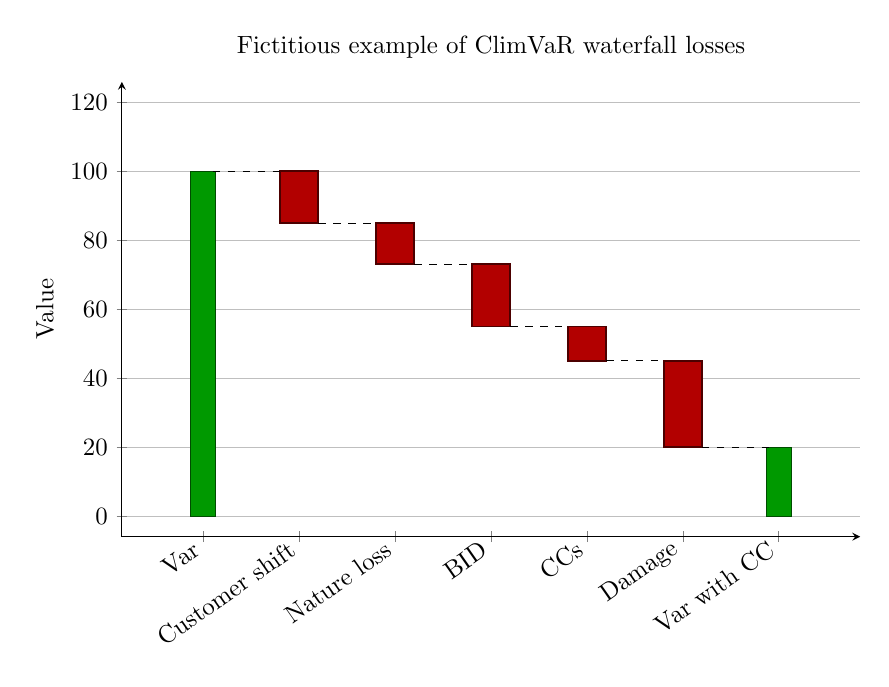
\begin{tikzpicture}[scale=0.9]
\begin{axis}[
    title={Fictitious example of ClimVaR waterfall losses},
    ylabel={Value},
    xmin=0.5, xmax=7.5,
    ymin=0, ymax=120,
    xtick={1,2,3,4,5,6,7},
    xticklabels={Var, Customer shift, Nature loss, BID, CCs, Damage, Var with CC},
    xticklabel style={rotate=35, anchor=east},
    xlabel style={yshift=-15pt},
    %xlabel={Steps},
    ymajorgrids,
    axis x line=bottom,
    axis y line=left,
    enlargelimits=0.05,
    ytick pos=left,
    width=12cm, height=8cm,
    clip=false,
]

% Initial blue bar: Var without CC (0 to 100)
\addplot[ ybar, fill=green!60!black, draw=green!30!black ] coordinates {(1,100)};

% Final blue bar: Var with CC (0 to 20)
\addplot[ ybar, fill=green!60!black, draw=green!30!black ] coordinates {(7,20)};

% Red waterfall bars with custom baselines using \fill
\fill[red!70!black] (axis cs:1.8,100) rectangle (axis cs:2.2,85);  % toto 1: 100→85
\fill[red!70!black] (axis cs:2.8,85)  rectangle (axis cs:3.2,73);  % toto 2: 85→73
\fill[red!70!black] (axis cs:3.8,73)  rectangle (axis cs:4.2,55);  % toto 3: 73→55
\fill[red!70!black] (axis cs:4.8,55)  rectangle (axis cs:5.2,45);  % toto 4: 55→45
\fill[red!70!black] (axis cs:5.8,45)  rectangle (axis cs:6.2,20);  % toto 5: 45→20

% Draw borders for red bars
\draw[red!30!black, thick] (axis cs:1.8,100) -- (axis cs:2.2,100) -- (axis cs:2.2,85) -- (axis cs:1.8,85) -- cycle;
\draw[red!30!black, thick] (axis cs:2.8,85)  -- (axis cs:3.2,85)  -- (axis cs:3.2,73) -- (axis cs:2.8,73) -- cycle;
\draw[red!30!black, thick] (axis cs:3.8,73)  -- (axis cs:4.2,73)  -- (axis cs:4.2,55) -- (axis cs:3.8,55) -- cycle;
\draw[red!30!black, thick] (axis cs:4.8,55)  -- (axis cs:5.2,55)  -- (axis cs:5.2,45) -- (axis cs:4.8,45) -- cycle;
\draw[red!30!black, thick] (axis cs:5.8,45)  -- (axis cs:6.2,45)  -- (axis cs:6.2,20) -- (axis cs:5.8,20) -- cycle;

% Cumulative floating lines
\draw[dashed, black] (axis cs:1.1,100) -- (axis cs:1.8,100);
\draw[dashed, black] (axis cs:2.2,85) -- (axis cs:2.8,85);
\draw[dashed, black] (axis cs:3.2,73) -- (axis cs:3.8,73);
\draw[dashed, black] (axis cs:4.2,55) -- (axis cs:4.8,55);
\draw[dashed, black] (axis cs:5.2,45) -- (axis cs:5.8,45);
\draw[dashed, black] (axis cs:6.2,20) -- (axis cs:6.9,20);
\end{axis}
\end{tikzpicture}
\end{center}


Equation (\ref{eq:central2}) allows to estimate all climate related losses, and we showed in the above figure the kind of analysis allowed by it. Equation (\ref{eq:var-without-cc}) allows to compare sectors between one another, and this could be done with a heatmap representations of all country sector combinations. 



\subsubsection{Company ClimVaR}

We consider a company as the sum of its $N_{_E}$ entities (belonging to a certain country $c$/sector $s$). The company valuation is then just the sum of its entity valuations
\begin{align}
V^{(C)}&=\sum_{E=1}^{N_{_E}}V^{(E)}_{_{cs}}\;.
\end{align}

\subsubsection{Financial porfolio ClimVaR}

ClimVaR trivially extent to a portfolio of financial $f$ products. In this context, the portfolio is just a weighted (weights being normalized sum invested in all $N_{_C}$ companies of the porfolio) sum of company Valuations. Calling $\theta_{_{FP,C}}$ the ratios of invested sums of financial portfolio $FP$ into company $C$, financial portfolio valuation reads
 \begin{align}
V^{(FP)}&=\sum_{C=1}^{N_{_C}}\theta_{_{FP,C}}V^{(C)}\;.
\end{align}

\subsubsection{Site ClimVaR}

Most of the analysis performed at entity level in section \ref{sec:climvar-entity} remain valid at site level. We consider an asset $a$ site belonging to coutry $c$ of sector $s$ in the following.  Changes are twofold. 

\vspace{0.2cm}

On the financial input terms:
\begin{itemize}
\item[•] Revenue is now specified at asset site level $Y_{_{a}}$.
\item[•] Asset value is now obviously specified at asset site level $AV_{_{a}}$.
\item[•] If it makes sense, growth rate $g$, tax rate $\tau$, weighted average cost of capital $\omega$, capex $k$, depreciation $d$, insurance premium $i$ are also adapted at site level. If no further information is provided, these information are taken from the entity the site belongs to.
\item[•] If available, COGS to revenue ratio $c$, OPEX to revenue ratio $o$, salary to Revenue ratio $s$, outdoor salary mass to revenue ratio $so$ and cooling costs $ec$ are taken from site specific data. If not available, entity information is used.
\end{itemize}
On the risk loss terms:
\begin{itemize}
\item[•] All physical losses are now obviously computed at site level: this means $\beta^{(t)}_{a}$,  $\xi^{(t)}_{a}$, $\gamma^{(t)}_{a}$ and $\delta^{(t)}_{a}$ are now computed at site level
\item[•] Nature loss $\rho^{(t)}_{a}$ is also obviously taken at site level.
\item[•] For carbon cost, scope 1 and 2 emissions should be known at site level. If not available, they could be deduce from revenues with carbon intentities. Purchases could also be known, but this is generally aggregated by an Enterprise Resource Planning (ERP) system at entity level. From all this we deduce individual $CC^{(ti)}_{_{a}}$
\end{itemize}
Future revenues taking into account climate change read\footnote{Customer shift is the only information that has to be taken from entity computation.}
\begin{align}
Y^{(t,cc)}_{_{a}}&=\left(1-\sigma^{(t)}_{_{cs}}\right)\left(1-\beta^{(t)}_{_{a}}\right)
%
\left(1-\rho^{(t)}_{_{a}}\right)Y^{(t)}_{_{a}}\;,
\end{align}

Our central equation (\ref{eq:central2}) then becomes
\begin{align}
\text{VAR}^{(S)}&=
%
\sum_{t=1}^{T+1}
%
\frac{\left( 1-\tau_{_{a}}\right)}{(1+\omega_{_{a}})^t}
%
\left[op_{_{a}}\left(Y_{_{a}}-Y^{(t,cc)}_{_{a}}\right)
%
+Y^{(t,cc)}_{_{a}}\left(so_{_{a}}\, \xi^{(t)}_{_{a}} + ec_{_{a}} \gamma^{(t)}_{_{a}}\right)
%
\right.\notag\\
%
&\left. +\sum_{i=1}^3CC^{(ti)}_{_{a}}+\left(1+i_{_{a}}\right) AV_{_{a}} \delta^{(t)}_{_{a}}
%
\right]\;.\label{eq:centralsite}
\end{align}


\subsubsection{Product ClimVaR}

Carefully computing ClimVaR at product level would require among other things to perform a LCA analysis for getting the detailed product carbon footprint. By doing so, all emissions generated by the product creation are correctly identified and associated to the countries in which they have been emitted and to the sectors of activities that were parts of the product supply chain in these countries. This changes drastically the carbon cost computation. 

\vspace{0.2cm} 

But most of the companies are not yet able to associate their purchases to specific products produced in specific sites. For this first study, we will therefore adopt another angle of attack.

\vspace{0.2cm}

A product could indeed be seen as a distribution given on sites, in the sense that several sites are needed to produce a product (but obviously a site can produce several products). So what is needed to perform a ClimVaR at product level of analysis is

\begin{itemize}
\item[$\bullet$] The part of a site $a$ revenue $\theta_{_{P,a}}$ associated to the product $P$
\item[$\bullet$] all these weights for all $N_{_a}$ sites contributing to producing $P$. 
\end{itemize}

ClimVaR at product level then reads

\begin{align}
\text{VAR}^{(P)}&=\sum_{a=1}^{N_{_a}} \theta_{_{P,a}} \text{VAR}^{(a)}
\end{align}
And reinjecting (\ref{eq:centralsite}) gives
\begin{align}
\text{VAR}^{(p)}&=\sum_{a=1}^{N_{_a}}\theta_{_P,a} \sum_{t=1}^{T+1}
%
\frac{\left( 1-\tau_{_{a}}\right)}{(1+\omega_{_{a}})^t}
%
\left[op_{_{a}}\left(Y_{_{a}}-Y^{(t,cc)}_{_{a}}\right)
%
+Y^{(t,cc)}_{_{a}}\left(so_{_{a}}\, \xi^{(t)}_{_{a}} + ec_{_{a}} \gamma^{(t)}_{_{a}}\right)
%
\right.\notag\\
%
&\left. +\sum_{i=1}^3CC^{(ti)}_{_{a}}+\left(1+i_{_{a}}\right) AV_{_{a}} \delta^{(t)}_{_{a}}
%
\right]\;.\label{eq:centralproduct}
\end{align}

Refinenement of the present approach will be the subject of future studies.


\subsection{Derivation of individual ClimVaR loss terms} \label{sec:climvar-terms}

The detailed derivation of each individual loss term---cooling penalty ($\gamma$), carbon costs (CC$^{1,2,3}$), business interruption ($\beta$), physical damage ($\delta$), and heat productivity ($\xi$)---follows the methodology established in \citet{epelbaum2025} and is not reproduced here. The core result is the entity-level ClimVaR formula presented in Section~\ref{sec:climvar-entity} and in the main text (Exhibit~6), where each channel maps to a specific cashflow line: $\gamma$, $\xi$, and CC affect COGS; $\beta$ affects revenue; and $\delta$ affects OPEX via insurance costs.

For the full mathematical derivation including the Shapley decomposition of hazard contributions and the Leontief input-output propagation of supply chain business interruption, we refer the reader to \citet{epelbaum2025}, Sections~3--5.

\subsection{Scenario} \label{sec:scenario}

Up to know we have avoided touching on the concept of climate scenario. This is a rich and quite complicated topic \cite{IPCCScenario} on its own, and we refer the reader to \cite{IPCCScenario}\cite{NGFS1} to learn more on the matter. Here we will just focus on a simple combined physical/nature/transition scenario. 

\subsubsection{Combining physical and transition scenarios} \label{sec:scenario-inter}

Physical climate scenarios go along the names of RCP2.5, 4.5, 8.5, SSP... For the present work, we just consider a low carbon scenario (RCP2.6 to fix ideas) and a high carbon one (RCP8.5).

\vspace{0.2cm}

For transition risks, NGFS \cite{NGFS1}\cite{NGFS2}\cite{NGFS3} has several scenarios (delayed transition, fragmented world...). We focus in our present study on Net Zero Transition (NZT) and Current Policies (CP).

\vspace{0.2cm}

We then easily form two ClimVaR $\nu$ scenarios:
\begin{itemize}
\item[•] An optimistic\footnote{Optimistic for the planet and its human inhabitants, though it might induce higher costs for emission intensive activities due to (among other things) carbon taxes.} one: Low Carbon for physical and NZT for transition
\item[•] A pessimistic one: High Carbon for physical and CP for transition 
\end{itemize}


To be noted, one could consider a worst case scenario with NZT for transition but high carbon for physical: it would correspond to a world where even though ambitious carbon mechanisms are put in place in the years to come, the carbon quantity in the atmoshpere does no decrease as fast as expected, due to high hysteresis physics ta we do not fully grasp yet (a hint on that is the regular underestimation of climate models on temperatures).

\subsubsection{Intra scenario uncertainty: link with usual VaR} \label{sec:scenario-intra}

While scenarios describe drastically different worlds, intra scenario uncertainty can be expressed in terms of the usual Value At Risk \cite{Jorion} (VaR). Up to know we have been using the word ClimVaR somewhat loosely, but we now make the connection between VaR and ClimVaR more clear.

\vspace{0.2cm}

While VaR has a rich history, it has been somewhat superseded by Conditional Value At Risk, or Expected Shorfall (ES) \cite{Artzner}-\cite{Rockafellar}. Indeed ES better captures the full tail of the loss distribution. We will therefore derive the connection for both VaR and ES.

\paragraph{Physical uncertainty related to ES} \label{sec:shortfall}

Let $e$ denote an extreme climatic event happening on an asset $a$ (flood, strong winds...). As briefly sketched in section \ref{sec:climvar-terms} physical quantities are derived from climate models\footnote{More on that in \cite{Popp}}. We will denote the climate models $m$. The future distribution of extreme events is givent by the  probability density function (pdf) $f(e \mid \bm{\theta}_{am})$, parameterized by the model-specific vector  $\bm{\theta}_{am} = (\theta_{a1m}, \ldots, \theta_{aIm})$ where $I$ is the number of parameters of the pdf. Examples of parameters: scale and shape for a Weibull distribution, location and scale for a Gumbell distribution or mean and variance for a Normal distribution.

\paragraph{ClimVaR physical risks as Mean Expected Values}

The different losses related to physical climate risks can be expressed a little more rigourously as follows. The expected effect of event $e$ at site $a$, applying the Law of the Unconscious Statistician (LOTUS), reads
\begin{align}
\mathbb{E}[D_s] &= \int D(e)\, f(e \mid \bar{\bm{\theta}}_a)\, \d e\;,  \label{eq:ed_s}
\end{align}
where $D(e)$ denotes the asset-level effect function (could be a damage function, a business interruption days function, or a CDD/HPL function as detailed in \citet{epelbaum2025}) and
\begin{align}
\bar{\bm{\theta}}_a &= \frac{1}{|M|}\sum_{m \in M} \bm{\theta}_{am}\;.  \label{eq:mean_theta}
\end{align}


Strictly speaking, the site-level expected damage should average over model-specific quantities $ g(\bm{\theta}_{am}) = \int D(e)f(e|\bm{\theta}_{am})\,d e$.
However, the approximation in \eqref{eq:ed_s} (evaluating at the mean parameters) is consistent with a first-order delta method expansion around $\bar{\bm{\theta}}_a$.

\vspace{0.2cm}

A country mean expected damage is then
\begin{align}
\mu &= \mathbb{E}[D]= \frac{1}{|A|}\sum_{a \in A} \mathbb{E}[D_a]. \label{eq:mean_country}
\end{align}
$\mu$ is then directly linked to the $(\beta,\delta,\xi,\gamma)_{_{cs}}$ that we derived in section \ref{sec:climvar-terms}.

\paragraph{Variance and Sources of Uncertainty}

Up to know the approach has been mostly deterministic, but different sources of uncertainties should be considered
\begin{itemize}
    \item (LOTUS) uncertainty, due to inherent event randomness.
    \item Uncertainty from variability among climate models.
    \item Spatial sampling uncertainty, due to finite coverage of sites across the country.
\end{itemize}

LOTUS uncertainty is straightforward
\begin{align}
\sigma_{1a}^2  &= \mathbb{V}(D_a) = \int D^2(e)\, f(e \mid \bar{\bm{\theta}}_a)\,\d e 
%
 - \big[\mathbb{E}(D_a)\big]^2\;,  \label{eq:sigma1s}
\end{align}
and veraging across assets leads to
\begin{align}
\sigma_1^2 = \frac{1}{|A|}\sum_{a \in A} \sigma_{1a}^2.
\label{eq:sigma1}
\end{align}
For model uncertainty, we define the covariance matrix among climate model parameters
\begin{align}
\bar{\Sigma}_{a,ij} &= \frac{1}{|M|-1}\sum_{m \in M} (\theta_{aim}-\bar{\theta}_{ai})(\theta_{ajm}-\bar{\theta}_{aj})\;. \label{eq:cov_theta}
\end{align}
Calling
\begin{align}
g(\bm{\theta}_a)  &= \int D(e)\, f(e \mid \bm{\theta}_a)\, \d e\;,\label{eq:g}
\end{align}
and using the delta method, the variance contribution from model-to-model spread is approximated by
\begin{align}
\sigma_{2a}^2 &= \nabla g(\bar{\bm{\theta}}_a)^{\!\top} \bar{\Sigma}_a\, 
%
\nabla g(\bar{\bm{\theta}}_a)\;,\label{eq:sigma2s}
\end{align}
where $\nabla g$ is the gradient column vector with respect to $\bm{\theta}_a$. Aggregating across assets gives
\begin{align}
\sigma_2^2 = \frac{1}{|A|}\sum_{a \in A} \sigma_{2a}^2. \label{eq:sigma2}
\end{align}
Spatial sampling uncertainty is straightforward to derive
\begin{align}
\sigma_3^2  &= \frac{1}{|A|-1}\sum_{a \in A} \big[\mathbb{E}(D_a) - \mu\big]^2\;. \label{eq:sigma3}
\end{align}
Assuming independence among the three uncertainty sources, we write the total uncertainty as
\begin{align}
\sigma^2 = \sigma_1^2 + \sigma_2^2 + \sigma_3^2\;,\label{eq:sigma_total}
\end{align}
keeping in mind that in our context $\sigma$ is really $\sigma_{_{cs}}$.

\paragraph{Value at Risk (VaR)}

The average effect $D$ of event $e$ at country sector level can be approximated by a Lognormal distribution (a more natural choice than a Gaussian since this effect is positive): $D \sim \text{LogNormal}(\mu_{\text{log}}, \sigma_{\text{log}})$, where $(\mu_{\text{log}}, \sigma_{\text{log}})$ are computed by standard moment matching:
\begin{align}
\mu_{\text{log}} &=  \ln\!\left(\frac{\mu}{\sqrt{1+\frac{\sigma^2}{\mu^2}}}\right), &
%
\sigma_{\text{log}} &= \sqrt{\ln\!\left(1+\frac{\sigma^2}{\mu^2}\right)}\;. \label{eq:mu_sigma_log}
\end{align}

For a given quantile level $ \lambda \in (0,1)$, the Value-at-Risk is the $1-\lambda$ quantile of the CDF of  $D$ and is therefore defined as
\begin{align}
\text{VaR}_\lambda &= F_D^{-1}(1-\lambda).
\end{align}
For a Lognormal distribution, this leads to the standard formula:
\begin{align}
\text{VaR}_\lambda &= \exp\!\big(\mu_{\text{log}} + \sigma_{\text{log}}\,\Phi^{-1}(1-\lambda)\big),
   \label{eq:VaR_lognormal}
\end{align}
where $ \Phi $ denotes the standard Normal cumulative distribution function (CDF).

\paragraph{Conditional Value-at-Risk (CVaR)/ Expected Shortfall (ES)}

ES \cite{Artzner}-\cite{Rockafellar} extends VaR by averaging all realizations exceeding the VaR threshold:
\begin{align}
\text{CVaR}_\lambda &= \frac{1}{\lambda}  \int_{1-\lambda}^{1} F_D^{-1}(u)\,\mathrm{d}u. 
%
= \frac{1}{\lambda} \int_{0}^{\lambda} F_D^{-1}(1-u)\,\mathrm{d}u
%
= \frac{1}{\lambda} \int_{0}^{\lambda} \text{VaR}_u \,\mathrm{d}u
\label{eq:CVaR_def}
\end{align}
For a Lognormal distribution, substituting \eqref{eq:VaR_lognormal} gives (This simple derivation is repeated in Appendix \ref{sec:appendix-es})
\begin{align}
\text{CVaR}_\lambda &= \frac{\exp\!\left(\mu_{\text{log}}+\frac{1}{2}\sigma_{\text{log}}^2\right)}{\lambda}
      \,\Phi\!\left(\sigma_{\text{log}} - \Phi^{-1}(1-\lambda)\right).
      \label{eq:CVaR_lognormal}
\end{align}

ClimVaR physical risks could then be evaluated in this sense. The treatment of uncertainty under multiple climate models is deferred to subsequent work.

\paragraph{Transition uncertainty}

Up to know we only considered average country sectors carbon intensities $I_{_{cs}}$. But these averages hide large variances: some virtuous actors have already started to reduce their emissions, change their energy mixes... While others still heavily relies on carbon intensive processes. 

\vspace{0.2cm}

We thus consider $I_{_{cs}}$  to be a pdf with a certain mean and variance, and follows the same logic as in the previous section \ref{sec:shortfall} to derive $I^{(\lambda)}_{_{cs}}$. This means that the carbon costs become\footnote{Please note that it is important to fix the denominator intensity for $EC$ in this intra scenario setup, otherwise $EC$ would not duly increase as the VaR/ES quantile considered increases.}
\begin{align}
MC^{(t\lambda)}_{_{cs}}&=\left[L \times \left(
%
\mathcal{C}^{(t)}\odot I^{(\lambda)}\right) \right]_{_{cs}}\;,&
%
EC^{(t\lambda)}_{_{cs}}&=\frac{\left[L \times \left(
%
 \mathcal{C}^{(t)}\odot I^{(\lambda)}\right) \right]_{_{cs}}}{\left[L \times
%
 I \right]_{_{cs}}}\;.
\end{align}

\subsubsection{Revised ClimVaR formula}



Formula (\ref{eq:central2}) can then be revised by adding to it the (inter/intra/ES) scenario concepts everywhere it makes sense, and clearly expressing all terms. 
 
\begin{tcolorbox}[colback=red!5!white,colframe=red!70!black,title=\textbf{Extended ClimVaR central $\text{VaR}^{(E\nu\lambda)}_{_{cs}}$ formula with scenarios },halign title=flush center]
\vspace{-0.4cm}
\begin{align}
&\sum_{t=1}^{T+1}\left[\underbrace{op_{_{cs}}\sigma^{(t\nu\lambda)}_{_{cs}}dY^{(t)}_{_{cs}}}_{\text{Customer Shift}}
%
+\underbrace{op_{_{cs}}\left(1-\sigma^{(t\nu\lambda)}_{_{cs}}\right) \beta^{(t\nu\lambda)}_{_{cs}}dY^{(t)}_{_{cs}}}_{\text{Business interruptions}}\right.\notag\\
%
&+\underbrace{op_{_{cs}}\left(1-\sigma^{(t\nu\lambda)}_{_{cs}}\right)\left(1-\beta^{(t\nu\lambda)}_{_{cs}}\right)  \rho^{(t\nu\lambda)}_{_{cs}}dY^{(t)}_{_{cs}}}_{\text{Renewable Natural Capital loss}}
%
+\underbrace{\left(1+i_{_{cs}}\right) \delta^{(t\nu\lambda)}_{_{cs}}dAV^{(t)}_{_{cs}}}_{\text{Asset Insurance premium}}\notag\\
%
&+\underbrace{s^{(1)}_{_{cs}}\mathcal{C}^{(t\nu\lambda)}_{_{cs}}dY^{(t\nu\lambda)}_{_{cs}}}_{\text{Scope 1 CC}}+
%
\underbrace{s^{(2)}_{_{cs_e}}EC^{(t\nu\lambda)}_{_{cs_e}}\left(1+  \varepsilon_{_{cs}}\gamma^{(t)}_{_{cs}}\right)dY^{(t\nu\lambda)}_{_{cs}}}_{\text{Scope 2 CC}}\notag\\
%
&\left. +\underbrace{p_{_{cs}}\mathcal{M}^{(t\nu\lambda)}_{_{cs}}dY^{(t\nu\lambda)}_{_{cs}}}_{\text{Scope 3 CC}}
%
+\underbrace{so_{_{cs}}\, \xi^{(t\nu\lambda)}_{_{cs}}dY^{(t\nu\lambda)}_{_{cs}}}_{\text{Heat Productivity Loss}}
%
+\underbrace{ec_{_{cs}} \gamma^{(t\nu\lambda)}_{_{cs}}dY^{(t\nu\lambda)}_{_{cs}}}_{\text{Cooling Cost Increase}}
%
\right. \Big]\;,\label{eq:central-scenar}
\end{align}
\end{tcolorbox}

where we have defined
\begin{align}
dY^{(t)}_{_{cs}}&= \frac{\left( 1-\tau_{_{cs}}\right)Y^{(t)}_{_{cs}}}{\left(1+\omega_{_{cs}}\right)^t}\;,&
%
dY^{(t\nu\lambda)}_{_{cs}}&=dY^{(t)}_{_{cs}}\frac{Y^{(t\nu\lambda,cc)}_{_{cs}}}{Y^{(t)}_{_{cs}}}\;,&
%
dAV^{(t)}_{_{cs}} &=   \frac{\left( 1-\tau_{_{cs}}\right)AV_{_{cs}}}{\left(1+\omega_{_{cs}}\right)^t} \;.
\end{align}


In a nutshell, ClimVaR then looks as follow

\vspace{0.2cm}

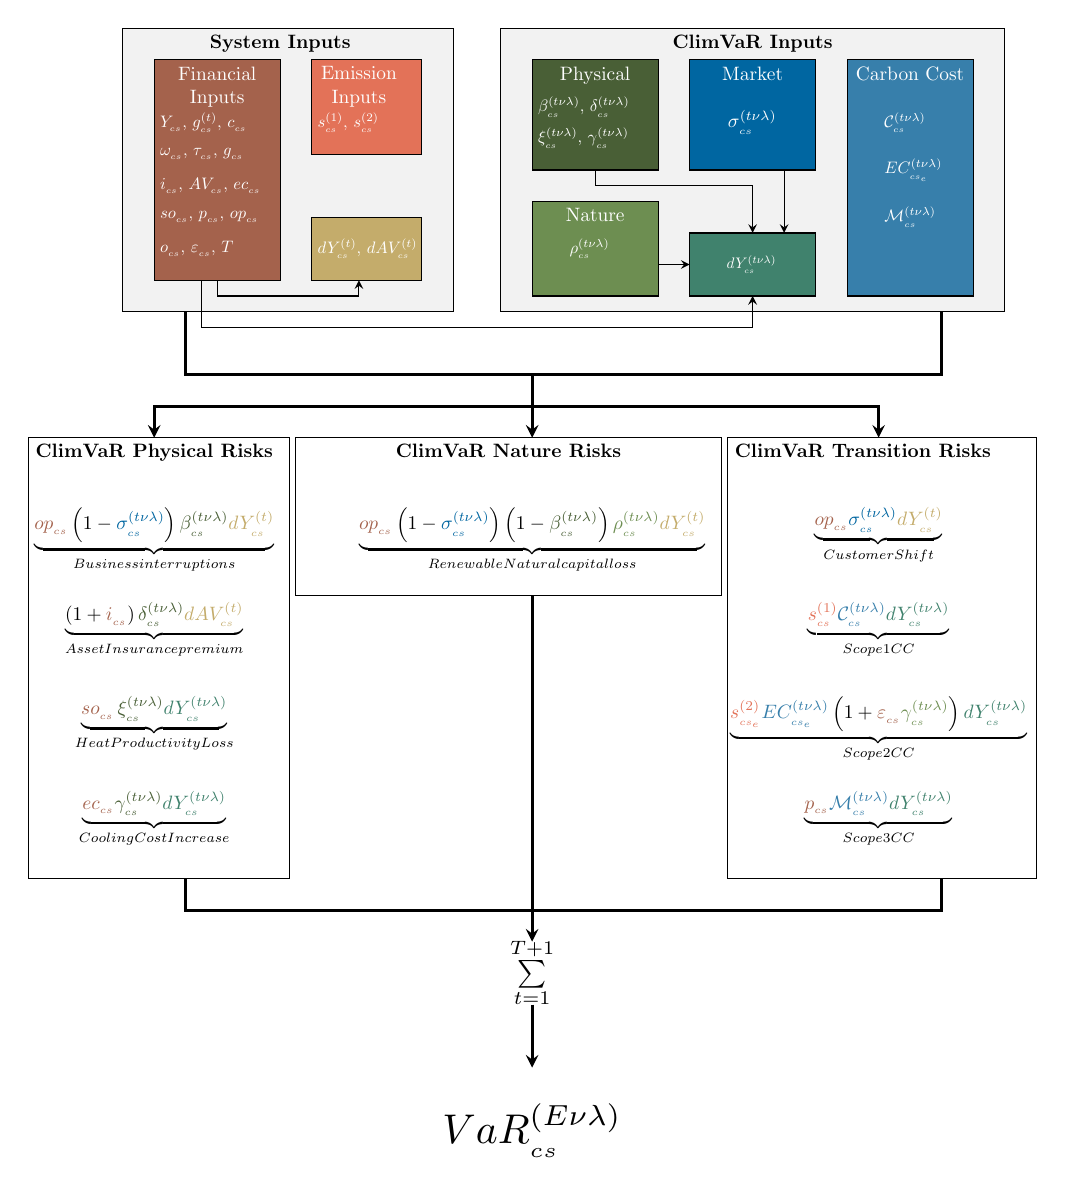
\begin{tikzpicture}[scale=0.8]
\filldraw[fill=gray!10!white,draw=black] (-10.5,-9) rectangle ++(5.25,4.5);
\node[anchor=north, align=center,scale=0.7] at (-8,-4.5) {\textbf{System Inputs}};
\filldraw[fill=gray!10!white,draw=black] (-4.5,-9) rectangle ++(8,4.5);
\node[anchor=north, align=center,scale=0.7] at (-0.5,-4.5) {\textbf{ClimVaR Inputs}};
\filldraw[fill=RED_PASTEL,draw=black] (-10,-8.5) rectangle ++(2,3.5);
\node[anchor=north, align=center,scale=0.7,color=white] at (-9,-5) {Financial\\ Inputs};
\node[anchor=west, align=center,scale=0.6,color=white,color=white] at (-10,-6) {$Y_{_{cs}}$, $g^{(t)}_{_{cs}}$, $c_{_{cs}}$};
\node[anchor=west, align=center,scale=0.6,color=white] at (-10,-6.5) {$\omega_{_{cs}}$, $\tau_{_{cs}}$, $g_{_{cs}}$};
\node[anchor=west, align=center,scale=0.6,color=white] at (-10,-7) {$i_{_{cs}}$, $AV_{_{cs}}$, $ec_{_{cs}}$};
\node[anchor=west, align=center,scale=0.6,color=white] at (-10,-7.5) {$so_{_{cs}}$, $p_{_{cs}}$, $op_{_{cs}}$};
\node[anchor=west, align=center,scale=0.6,color=white] at (-10,-8) {$o_{_{cs}}$, $\varepsilon_{_{cs}}$, $T$};
\filldraw[fill=RED_MAIN,draw=black] (-7.5,-6.5) rectangle ++(1.75,1.5);
\node[anchor=north, align=center,scale=0.7,color=white] at (-6.75,-5) {Emission\\Inputs};
\node[anchor=west, align=center,scale=0.6,color=white] at (-7.5,-6) {$s^{(1)}_{_{cs}}$, $s^{(2)}_{_{cs}}$};
\filldraw[fill=RED_DARK,draw=black] (-7.5,-8.5) rectangle ++(1.75,1);
\node[anchor=west, align=center,scale=0.6,color=white] at (-7.5,-8) {$dY^{(t)}_{_{cs}}$, $dAV^{(t)}_{_{cs}}$};
\draw[-stealth] (-9,-8.5) -- (-9,-8.75) -- (-6.75,-8.75) -- (-6.75,-8.5);
\filldraw[fill=GREEN_DARKER,draw=black] (-4,-6.75) rectangle ++(2,1.75);
\node[anchor=north, align=center,scale=0.7,color=white] at (-3,-5) {Physical};
\node[anchor=west, align=center,scale=0.6,color=white] at (-4,-5.75) {$\beta^{(t\nu\lambda)}_{_{cs}}$, $\delta^{(t\nu\lambda)}_{_{cs}}$};
\node[anchor=west, align=center,scale=0.6,color=white] at (-4,-6.25) {$\xi^{(t\nu\lambda)}_{_{cs}}$, $\gamma^{(t\nu\lambda)}_{_{cs}}$};
\filldraw[fill=GREEN_DARK,draw=black] (-4,-8.75) rectangle ++(2,1.5);
\node[anchor=north, align=center,scale=0.7,color=white] at (-3,-7.25) {Nature};
\node[anchor=west, align=center,scale=0.6,color=white] at (-3.5,-8) {$\rho^{(t\nu\lambda)}_{_{cs}}$};
\filldraw[fill=BLUE_MAIN,draw=black] (-1.5,-6.75) rectangle ++(2,1.75);
\node[anchor=north, align=center,scale=0.7,color=white] at (-0.5,-5.) {Market};
\node[anchor=west, align=center,scale=0.7,color=white] at (-1,-6) {$\sigma^{(t\nu\lambda)}_{_{cs}}$};
\filldraw[fill=GREEN_REL,draw=black] (-1.5,-8.75) rectangle ++(2,1);
\node[anchor=west, align=center,scale=0.55,color=white] at (-1,-8.25) {$dY^{(t\nu\lambda)}_{_{cs}}$};
\draw[-stealth] (-2,-8.25) -- (-1.5,-8.25);
\draw[-stealth] (-0,-6.75) -- (-0,-7.75);
\draw[-stealth] (-3,-6.75) -- (-3,-7) -- (-0.5,-7) -- (-0.5,-7.75);
\draw[-stealth] (-9.25,-8.5) -- (-9.25,-9.25) -- (-0.5,-9.25) -- (-0.5,-8.75);
\filldraw[fill=BLUE_PASTEL,draw=black] (1,-8.75) rectangle ++(2,3.75);
\node[anchor=north, align=center,scale=0.7,color=white] at (2,-5.) {Carbon Cost};
\node[anchor=west, align=center,scale=0.6,color=white] at (1.5,-6) {$\mathcal{C}^{(t\nu\lambda)}_{_{cs}}$};
\node[anchor=west, align=center,scale=0.6,color=white] at (1.5,-6.75) {$EC^{(t\nu\lambda)}_{_{cs_e}}$};
\node[anchor=west, align=center,scale=0.6,color=white] at (1.5,-7.5) {$\mathcal{M}^{(t\nu\lambda)}_{_{cs}}$};
%TODO: add \mathcal{M}^{(t\nu\lambda)}_{_{cs}} BELOW A matrix
\draw[-stealth,line width=1pt] (-9.5,-9) -- (-9.5,-10) -- (-4,-10) -- (-4,-10.5)  -- (-10,-10.5)  -- (-10,-11) ;
\draw[-stealth,line width=1pt] (2.5,-9) -- (2.5,-10) -- (-4,-10) -- (-4,-10.5)  -- (1.5,-10.5)  -- (1.5,-11);
\draw[-stealth,line width=1pt] (-4,-10.5)  -- (-4,-11);
%
\filldraw[fill=white,draw=black] (-12,-18) rectangle ++(4.15,7);
\node[anchor=north, align=center,scale=0.7] at (-10,-11) {\textbf{ClimVaR Physical Risks}};
%
\filldraw[fill=white,draw=black] (-7.75,-13.5) rectangle ++(6.75,2.5);
\node[anchor=north, align=center,scale=0.7] at (-4.375,-11) {\textbf{ClimVaR Nature Risks}};
%
\filldraw[fill=white,draw=black] (-0.9,-11) -- (-0.9,-14.75) -- (-0.9,-14.75) --(-0.9,-16) --(-0.9,-16)  --(-0.9,-18)-- (4,-18) -- (4,-16) -- (4,-16) -- (4,-14.75)-- (4,-14.75) -- (4,-11) --  (-0.9,-11);
\node[anchor=north, align=center,scale=0.7] at (1.25,-11) {\textbf{ClimVaR Transition Risks}};
%
\node[anchor=north, align=center,scale=0.7] at (-10,-12) {$\underbrace{\textcolor{RED_PASTEL}{op_{_{cs}}}\left(1-\textcolor{BLUE_MAIN}{\sigma^{(t\nu\lambda)}_{_{cs}}}\right) \textcolor{GREEN_DARKER}{\beta^{(t\nu\lambda)}_{_{cs}}}\textcolor{RED_DARK}{dY^{(t)}_{_{cs}}}}_{\text{Business interruptions}}$};
%
\node[anchor=north, align=center,scale=0.7] at (-10,-13.5) {$\underbrace{\left(1+\textcolor{RED_PASTEL}{i_{_{cs}}}\right)\textcolor{GREEN_DARKER}{\delta^{(t\nu\lambda)}_{_{cs}}} \textcolor{RED_DARK}{dAV^{(t)}_{_{cs}}}}_{\text{Asset Insurance premium}}$};
%
\node[anchor=north, align=center,scale=0.7] at (-10,-15) {$\underbrace{\textcolor{RED_PASTEL}{so_{_{cs}}}\, \textcolor{GREEN_DARKER}{\xi^{(t\nu\lambda)}_{_{cs}}} \textcolor{GREEN_REL}{ dY^{(t\nu\lambda)}_{_{cs}}}}_{\text{Heat Productivity Loss}}$};
%
\node[anchor=north, align=center,scale=0.7] at (-10,-16.5) {$\underbrace{\textcolor{RED_PASTEL}{ec_{_{cs}}} \textcolor{GREEN_DARKER}{\gamma^{(t\nu\lambda)}_{_{cs}}} \textcolor{GREEN_REL}{ dY^{(t\nu\lambda)}_{_{cs}}}}_{\text{Cooling Cost Increase}}$};
%
\node[anchor=north, align=center,scale=0.7] at (-4,-12) {$\underbrace{\textcolor{RED_PASTEL}{op_{_{cs}}}\left(1-\textcolor{BLUE_MAIN}{\sigma^{(t\nu\lambda)}_{_{cs}}}\right)\left(1-\textcolor{GREEN_DARKER}{\beta^{(t\nu\lambda)}_{_{cs}}}\right)  \textcolor{GREEN_DARK}{\rho^{(t\nu\lambda)}_{_{cs}}}\textcolor{RED_DARK}{dY^{(t)}_{_{cs}}}}_{\text{Renewable Natural capital loss}}$};
%
\node[anchor=north, align=center,scale=0.7] at (1.5,-12) {$\underbrace{\textcolor{RED_PASTEL}{op_{_{cs}}}\textcolor{BLUE_MAIN}{\sigma^{(t\nu\lambda)}_{_{cs}}}\textcolor{RED_DARK}{dY^{(t)}_{_{cs}}}}_{\text{Customer Shift}}$};
%
\node[anchor=north, align=center,scale=0.7] at (1.5,-13.5) {$\underbrace{\textcolor{RED_MAIN}{s^{(1)}_{_{cs}}}\textcolor{BLUE_PASTEL}{\mathcal{C}^{(t\nu\lambda)}_{_{cs}}}\textcolor{GREEN_REL}{ dY^{(t\nu\lambda)}_{_{cs}}}}_{\text{Scope 1 CC}}$};
%
\node[anchor=north, align=center,scale=0.7] at (1.5,-15) {$\underbrace{\textcolor{RED_MAIN}{s^{(2)}_{_{cs_e}}} \textcolor{BLUE_PASTEL}{EC^{(t\nu\lambda)}_{_{cs_e}}}\left(1+\textcolor{RED_PASTEL}{\varepsilon_{_{cs}}} \textcolor{GREEN_DARK}{\gamma^{(t\nu\lambda)}_{_{cs}}} \right)\textcolor{GREEN_REL}{ dY^{(t\nu\lambda)}_{_{cs}}}}_{\text{Scope 2 CC}}$};
%
\node[anchor=north, align=center,scale=0.7] at (1.5,-16.5) {$\underbrace{\textcolor{RED_PASTEL}{p_{_{cs}}}\textcolor{BLUE_PASTEL}{\mathcal{M}^{(t\nu\lambda)}_{_{cs}}}\textcolor{GREEN_REL}{ dY^{(t\nu\lambda)}_{_{cs}}}}_{\text{Scope 3 CC}}$};
\draw[-stealth,line width=1pt] (-9.5,-18) -- (-9.5,-18.5) -- (-4,-18.5) -- (-4,-19);
\draw[line width=1pt] (-4,-13.5) -- (-4,-18.5);
\draw[line width=1pt] (2.5,-18) -- (2.5,-18.5) -- (-4,-18.5);
\node[align=center] at (-4,-19.5) {$\sum\limits_{t=1}^{T+1}$};
%
\draw[-stealth,line width=1pt] (-4,-20) -- (-4,-21);
\node[align=center,scale=1.5] at (-4,-22) {$\text{VaR}^{(E\nu\lambda)}_{_{cs}}$};
\end{tikzpicture}






\subsection{Expected Shortfall for a lognormal distribution} \label{sec:appendix-es}


Starting from \eqref{eq:CVaR_def} and using \eqref{eq:VaR_lognormal},
\begin{align}
\text{CVaR}_\lambda
%
&= \frac{1}{\lambda}\int_0^{\lambda}\exp\!\big(\mu_{\text{log}} + \sigma_{\text{log}}\Phi^{-1}(1-\gamma)\big)\,\mathrm{d}\gamma\notag\\
%
 &= \frac{1}{\lambda}\int_{1-\lambda}^{1} 
     \exp\!\big(\mu_{\text{log}} + \sigma_{\text{log}}\Phi^{-1}(\gamma)\big)\, \mathrm{d}\gamma.
\end{align}
With the variable substitution $ \gamma = \Phi(x)$, 
we have $ \d\gamma = \phi(x)\,\d x = \frac{1}{\sqrt{2\pi}} e^{-x^2/2}\d x$, leading to
\begin{align}
\text{CVaR}_\lambda
 &= \frac{e^{\mu_{\text{log}}}}{\sqrt{2\pi}\lambda}
    \int_{\Phi^{-1}(1-\lambda)}^{+\infty}
       e^{\sigma_{\text{log}}x}e^{-x^2/2}\,\mathrm{d}x  \\[3pt]
 &= \frac{e^{\mu_{\text{log}}+\frac{1}{2}\sigma_{\text{log}}^2}}{\sqrt{2\pi}\lambda}
    \int_{\Phi^{-1}(1-\lambda)-\sigma_{\text{log}}}^{+\infty}
       e^{-x^2/2}\,\mathrm{d}x \\[3pt]
        &= \frac{e^{\mu_{\text{log}}+\frac{1}{2}\sigma_{\text{log}}^2}}{\sqrt{2\pi}\lambda}
    \int^{\sigma_{\text{log}}-\Phi^{-1}(1-\lambda)}_{-\infty}
       e^{-x^2/2}\,\mathrm{d}x \\[3pt]
 &= \frac{e^{\mu_{\text{log}}+\frac{1}{2}\sigma_{\text{log}}^2}}{\lambda}
    \,\Phi\!\left(\sigma_{\text{log}}-\Phi^{-1}(1-\lambda)\right),
\end{align}
which confirms the closed-form expression in \eqref{eq:CVaR_lognormal}.





